%task

%scheduling
%classification
%-preemtion
%-non-preemtion
%-dynamic
%-static
%-online
%periodic
%schedubility test

%constraint
%-timming
%-resource
%share resource
%problem
%solution (resource constarint)

\section{Background}
In this section, we will describe the concept and terms that are dominant in this research paper.

\subsection{Task}

According to \cite{b4}- "a Task is a sequence of instructions that, in the absence of other activities, is continuously executed by the processor until completion."

Task, thread, job and process  are the basic component in task scheduling. At the level of scope of this paper, the term process and thread have the same definition as task. 

An example of a task could be writing or reading a variable's value. Some task have its instance called Job as defined in \cite{b4}-"Job is an instance of a task executed on a specific input data". 

Next I will explain how tasks are executed.


\subsection{Scheduling Policy and Scheduling Algorithm }


In real time system, more than one task that are concurrent, are handled even in system with uni-processor. To realize it,  the task are executed in order using a defined algorithm called scheduling algorithm. For that reasons many scheduling algorithm have been proposed such as Earliest Deadline First, The Earliest Deadline Late serve and many more. The task is ordered by assigning their priority through set of predefined criterion called scheduling policy.

Considering that the schedule algorithm handles more than one task, now we will extend the definition of a task to correspond to their state as listed in the list below.

\begin{itemize}
\item A task that could potentially execute on the CPU can be either in execution (if it has been selected by the scheduling algorithm) or waiting for the CPU (if another task is executing)\cite{b5}.

\item A task that can potentially execute on the processor, independently of its actual availability, is called an active task\cite{b5}.

\item A task waiting for the processor is called a ready task, whereas the task in execution is called a running task\cite{b5}.

\item All ready tasks waiting for the processor are kept in a queue, called ready queue\cite{b5}.

\end{itemize}

Scheduling Algorithms are built to solve a curtain problem for a curtain environment. Means that they can be classified base on their characteristic. The classification of the algorithm will be explained in the next sub topic

\subsection{Classification of Scheduling Algorithms}

In this subtopic, we will only focus on important classification of scheduling algorithm that are related to the scope of this research paper, which is resource access protocols that will be discussed in resource access protocol section. 

\begin{itemize}
\item Preemptive: running task can be interrupted at any time\cite{b5}.
\item Non-preemptive: a task, once started, is executed until completion\cite{b5}.
\item Static: scheduling decisions are based on fixed parameters (off-line)\cite{b5}.
\item Dynamic: scheduling decisions are based on parameters that change during system evolution\cite{b5}.
\item Off-line : Scheduling algorithm is performed on the entire task set before start of system. Calculated schedule is executed by dispatcher\cite{b5}. 
\item On-line : scheduling decisions are taken at run-time every time a task enters or leaves the system\cite{b5}.
\item Optimal : the algorithm minimizes some given cost function, alternatively : it may fail to meet a deadline only if no other algorithm of the same class can meet it\cite{b5}.
\item Heuristic : algorithm that tends to find the optimal schedule, but does not guarantee to find it\cite{b5}.
\end{itemize}

In real time system not only the characteristic of algorithm are matter but also the characteristics  of task that being handle by scheduling algorithm, such as periodic and aperiodic that will be discussed in the next subtopic.

\subsection{Periodic and Aperiodic Task}

A task can be periodic or aperiodic, base on the way it is activated. Their definition is listed below \cite{b4}
\begin{itemize}
\item Periodic Task: a task in which jobs are activated at regular intervals of time, such that the activation of consecutive jobs is separated by a fixed interval of time, called the task period\cite{b4}.
\item Aperiodic Task: a task in which jobs may be activated at arbitrary time intervals\cite{b4}.
\end{itemize}

The task characteristic that handled by the resource access protocol that we will discuss later is limited to periodic tasks. Figure \ref{fig:periodic} shows an example of periodic task. As explained before, a scheduling algorithm is used to handle a many tasks by executing them in order based on their priority. The priority is influenced by the constraint that they have. Next,  I will explain some of important task constraint

\begin{figure}[h]
    \centering
    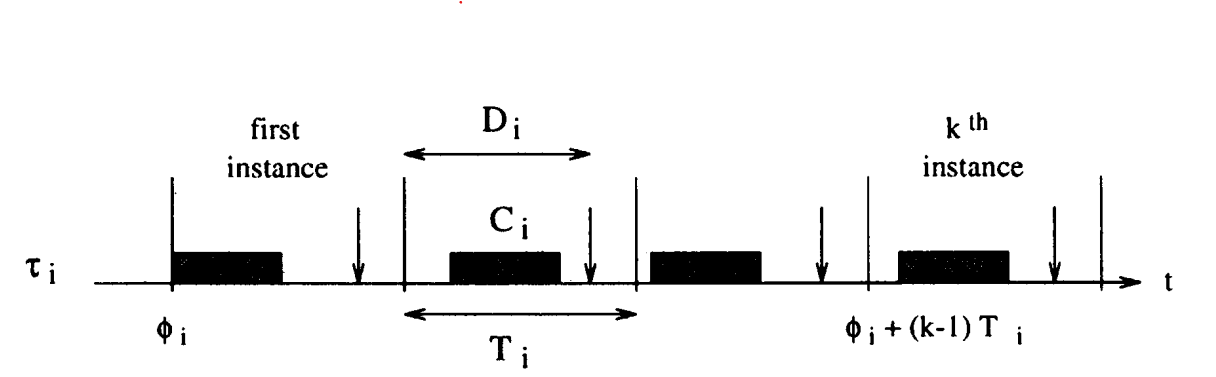
\includegraphics[width=0.5\textwidth]{periodic}
    \caption{periodic task \cite{b5}}
    \label{fig:periodic}
\end{figure}

\subsection{Task Constraint}

Task constraints are rules that are used by the scheduling algorithm to set  priority for each task. There are 3 main type of task constraint, and they are:

\begin{itemize}
\item Timing constraint
\item Precedence constraint
\item Resource constraint
\end{itemize}

Next we will explain more detail about timing constraint and resource constraint and how they are related to this paper topic. Precedence constraint is not covered in this paper. 

\subsubsection{Timing Constraint}

One of the timing constraint that are essential in this paper is deadline. There is two type of deadline:
\begin{itemize}
\item Relative Deadline: the longest interval of time within which any job should complete its execution\cite{b4}.
\item Absolute Deadline (of a job): the time at which a specific job should complete its execution\cite{b4}.
\end{itemize}

The deadline of a task or job could be missed if concurrent tasks are not well handled. For that reasons, we should ensure that our real time system is well predicted. This is why we have another constraints including resource constraint that will be explained in the next subsection to solve the problem regarding the predictability of the system. With time constraint we also can characterize real time system into three categories :
\begin{itemize}
\item Hard Real Time System - failed to meet the deadline can cause catastrophic event 
\item Soft Real Time System - failed to meet the deadline only cause the degradation of the system 
\item Firm Real Time System - failed to meet the deadline only cause the production of useless output 
\end{itemize}
Hard real time is the main focus in this research paper.

\subsubsection{Resource Constraint}

As mentioned before, another important constraint related to this topic is resource constraint. First, we need to understand what resource means in this paper.

According to \cite{b5} - "resource is any software structure that can be used by the process to advance its execution. Typically, a resource can be a data structure, a set of variables, a main memory area, a file, a piece of program, or a set of registers of a peripheral device. A resource dedicated to a particular process is said to be private, whereas a resource that can be used by more tasks is called a shared resource. A shared resource protected against concurrent accesses is called an exclusive resource."


Resource constraint that we are focus on is the mechanism that avoid more than one concurrent tasks to access an exclusive resource at the same time. Figure \ref{fig:Two_tasks_sharing} shows an example of resource, R that holding the value $x$ and $y$ and two tasks $\tau_{W}$ and $\tau_{D}$ with their critical sections. In general, concurrent tasks are not allowed to access shared resources at the same time to avoid data inconsistency, as illustrated in Figure \ref{fig:Example_of_schedule_creating_data_inconsistency}. Now, the value of $x$ and $y$ in critical section of $\tau_{D}$ is 4 and 2 instead of 4 and 8.

\begin{figure}[h]
    \centering
    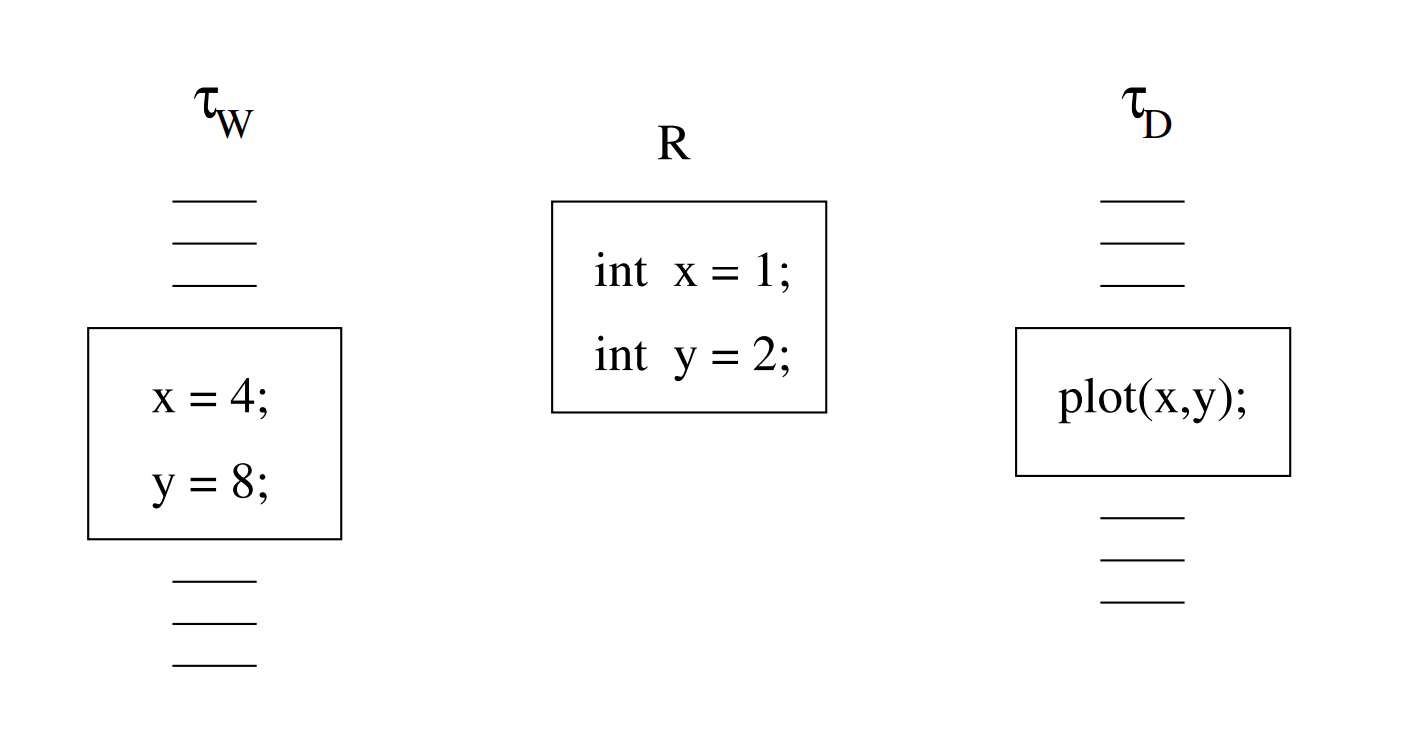
\includegraphics[width=0.5\textwidth]{Two_tasks_sharing}
    \caption{ Two tasks sharing a buffer with two variables. \cite{b5}}
    \label{fig:Two_tasks_sharing}
\end{figure}

\begin{figure}[h]
    \centering
    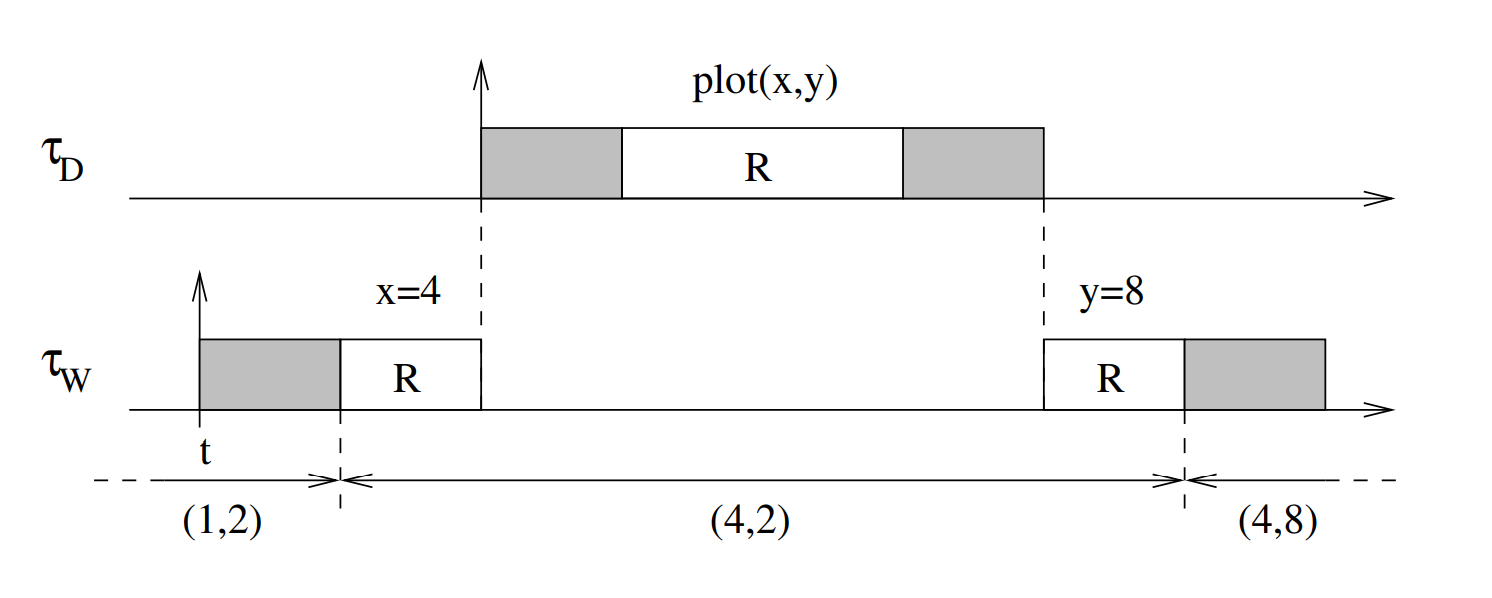
\includegraphics[width=0.5\textwidth]{Example_of_schedule_creating_data_inconsistency}
    \caption{Example of schedule creating data inconsistency. \cite{b5}}
    \label{fig:Example_of_schedule_creating_data_inconsistency}
\end{figure}


To avoid this situation, various synchronization mechanism had been invented such as\textit{Semaphore}. In this mechanism, each critical section must begin with wait(s) primitive and end with signal(s) primitive, where s is a binary semaphore as shown in Figure \ref{fig:Structure} and due to this mechanism, the state of a task can be extended as shown in Figure \ref{fig:state}. Means that a task cannot access an exclusive resource if another task currently accessing the resource until signal(s) is executed. This mechanism can ensure the data consistency as illustrated in Figure \ref{fig:semaphore}. For the sake of simplicity, in this paper, we use the word resource for exclusive resource. 

\begin{figure}[h]
    \centering
    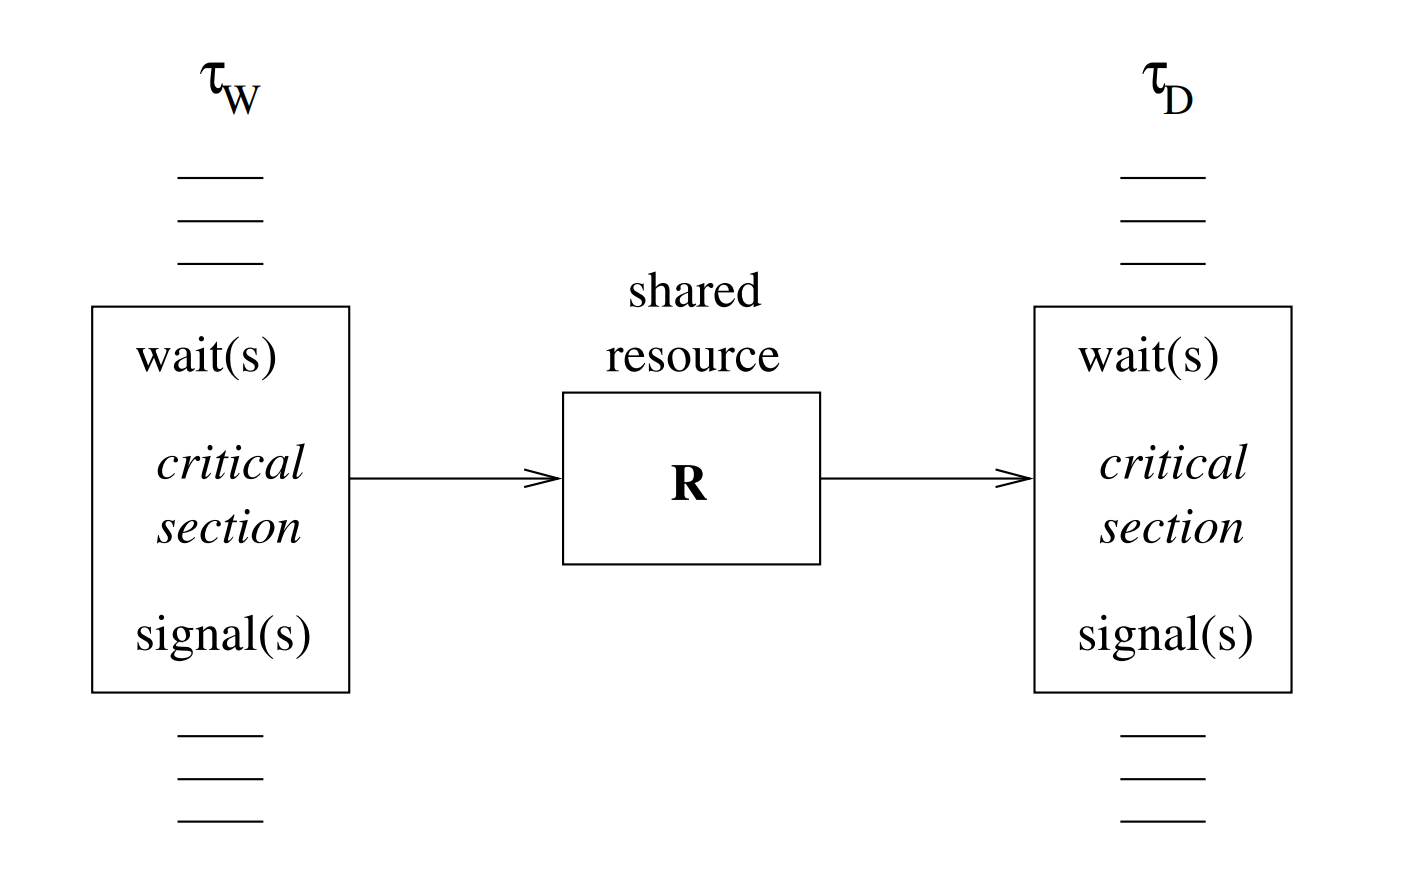
\includegraphics[width=0.5\textwidth]{Structure}
    \caption{Structure of two tasks that share a mutually exclusive resource protected by
a semaphore. \cite{b5}}
    \label{fig:Structure}
\end{figure}


\begin{figure}[h]
    \centering
    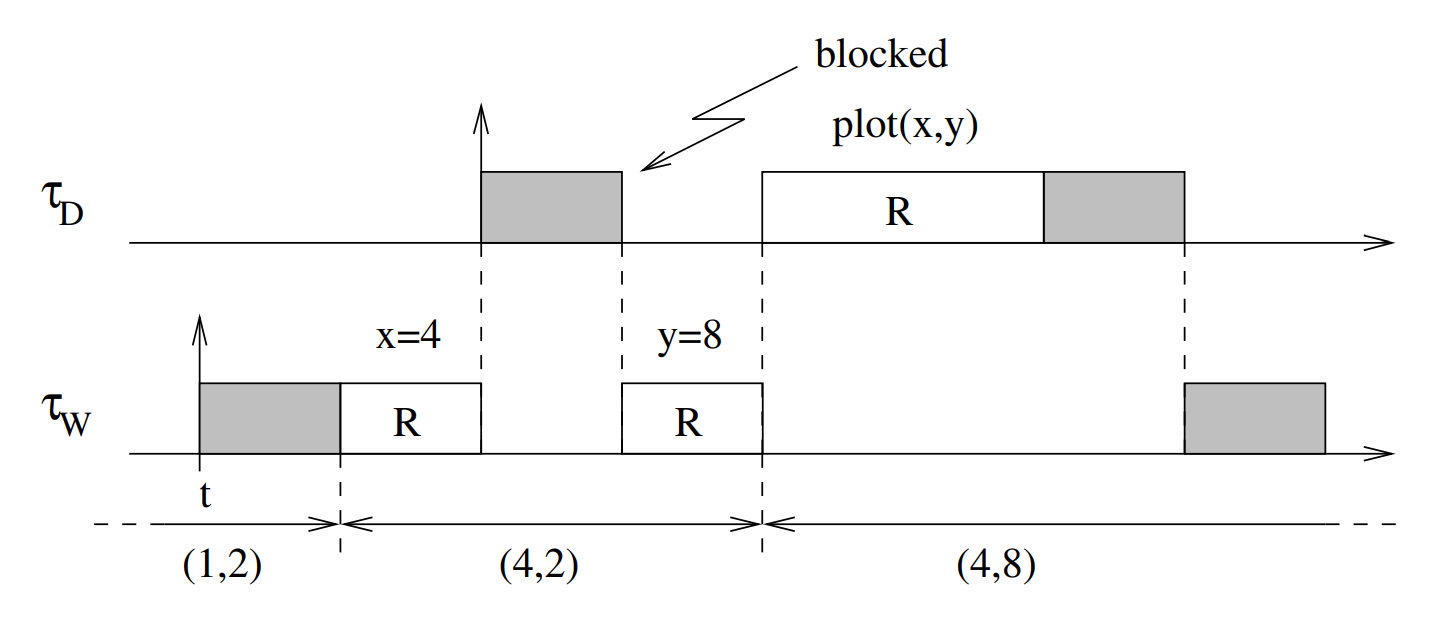
\includegraphics[width=0.5\textwidth]{semaphore}
    \caption{Example of schedule when the resource is protected by a semaphore.. \cite{b5}}
    \label{fig:semaphore}
\end{figure}

\begin{figure}[h]
    \centering
    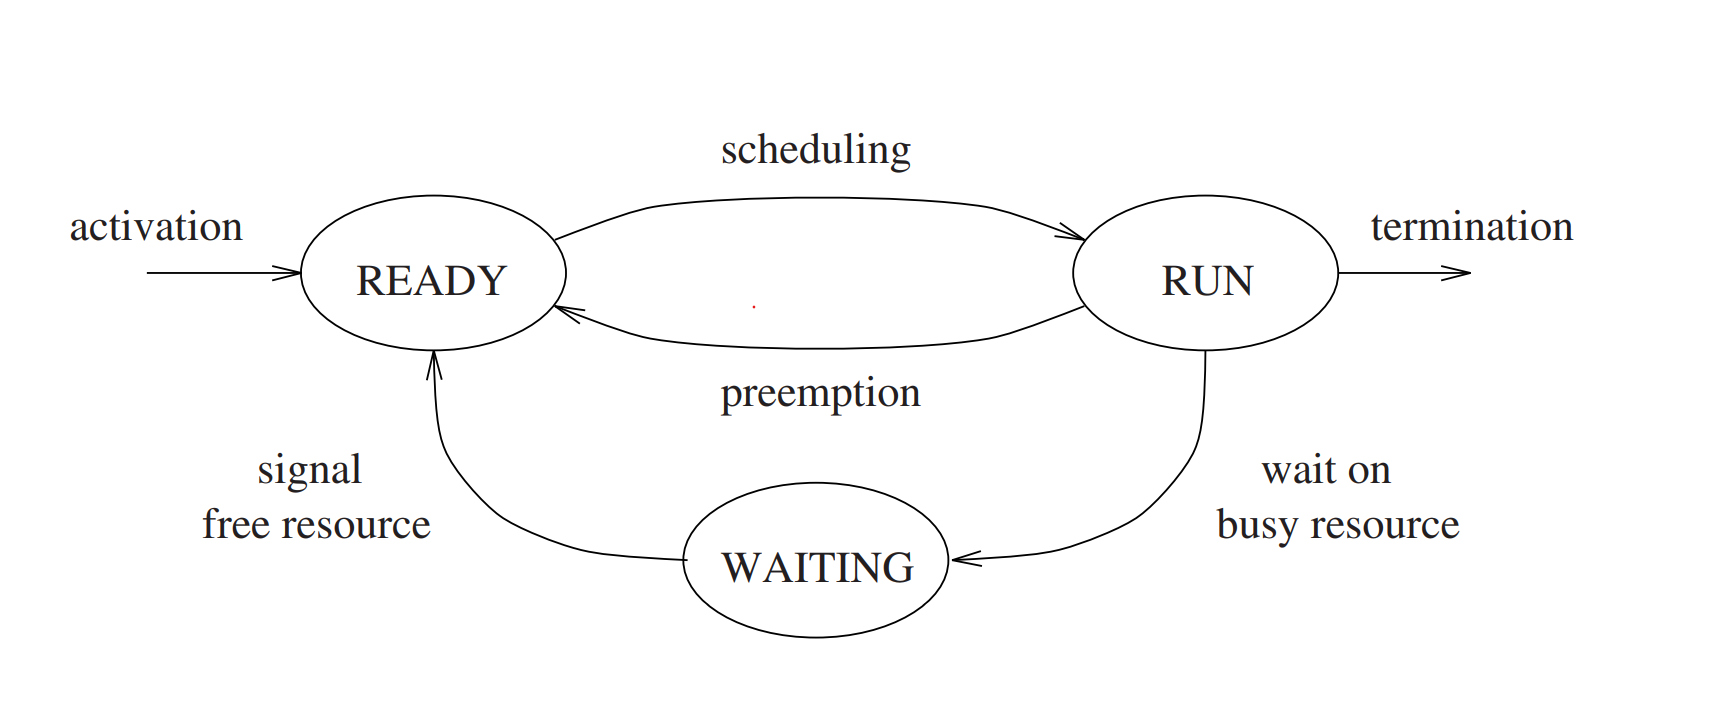
\includegraphics[width=0.5\textwidth]{state}
    \caption{Waiting state caused by resource constraints. \cite{b5}}
    \label{fig:state}
\end{figure}



\subsection{Schedulability}

Before we are considering implementing resource access protocol, it is important to make sure that all task are schedulable or a schedule is feasible on the set of task. This can be done through scheduability test. This paper will not explain about scheduability test since all task already considered as schedulable. More detail about scheduability test can be found in \cite{b5}.

In the next section, we will discuss arose problem due to proposed synchronization mechanism that affect the predictability of a real time system.